\documentclass[12pt]{article}
\usepackage[margin=1in]{geometry} 
\usepackage{amsmath,amsthm,amssymb,amsfonts}
\usepackage{graphicx}
\usepackage{float}
\newcommand{\N}{\mathbb{N}}
\newcommand{\Z}{\mathbb{Z}}
\newenvironment{problem}[2][Problem]{\begin{trivlist}
		\item[\hskip \labelsep {\bfseries #1}\hskip \labelsep {\bfseries #2.}]}{\end{trivlist}}
\begin{document}
	\begin{figure}[h]
		\centering
		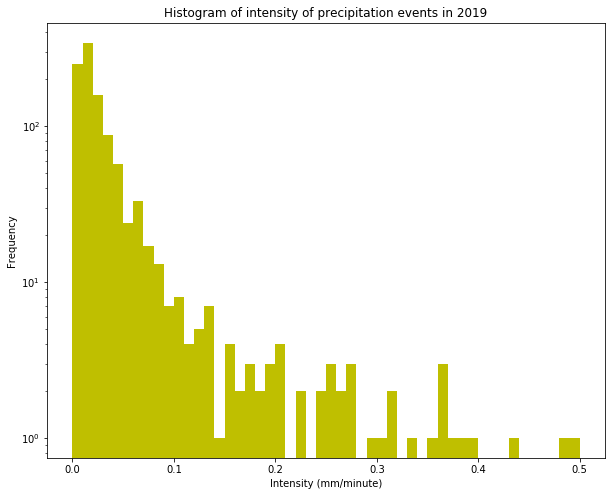
\includegraphics[width=150mm]{intensity_hist_5min.png}
		\caption{This is a histogram of intensity of precipitation events, in which the intensity is the total precipitation of a precipitation event divided by the duration of the precipitation event. We can see the distribution decrease logarithmically as we got from 0.01 mm/minute to 0.5 mm/minute in intensity.}
	\end{figure}
	\begin{figure}[h]
	\centering
	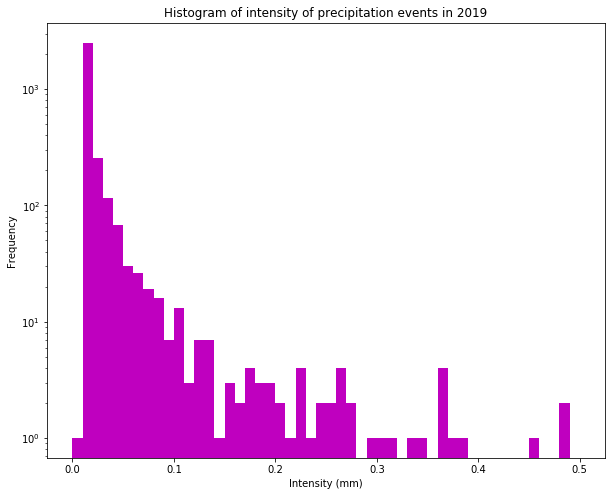
\includegraphics[width=150mm]{intensity_hist_1min.png}
	\caption{This is a histogram of intensity of precipitation events in which the minimum precipitation event duration is set to 1 minute, in which the intensity is the total precipitation of a precipitation event divided by the duration of the precipitation event. It is clear to see lots of intensity of precipitation events are near 0.01 mm/minute.}
\end{figure}
\begin{figure}[h]
	\centering
	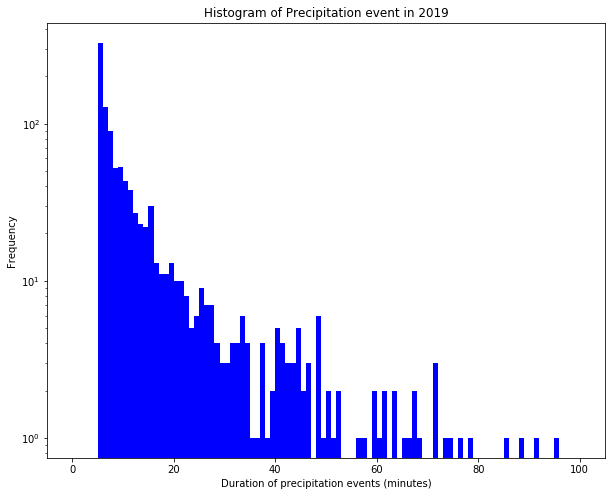
\includegraphics[width=150mm]{precip_hist_5min.png}
	\caption{A histogram that shows the duration of precipitation event. Note that in this histogram that the 5 minutes was the minimum duration needed to define a precipitation event. As expected, the distribution is that we have most precipitation events be close to the minimum duration and that less precipitation events are particularly long. }
\end{figure}
\begin{figure}[h]
	\centering
	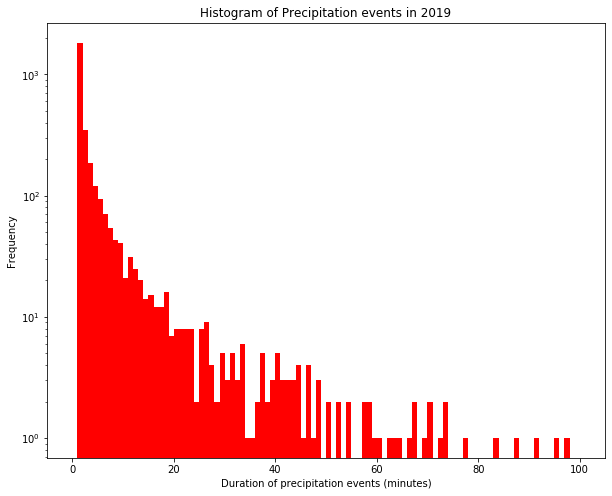
\includegraphics[width=150mm]{precip_hist_1min.png}
	\caption{A histogram that shows the duration of precipitation event. Note that in this histogram that the 1 minute was the minimum duration needed to define a precipitation event. As expected, the distribution is that we have most precipitation events be close to the minimum duration and that less precipitation events are particularly long. }
\end{figure}
\begin{figure}[h]
	\centering
	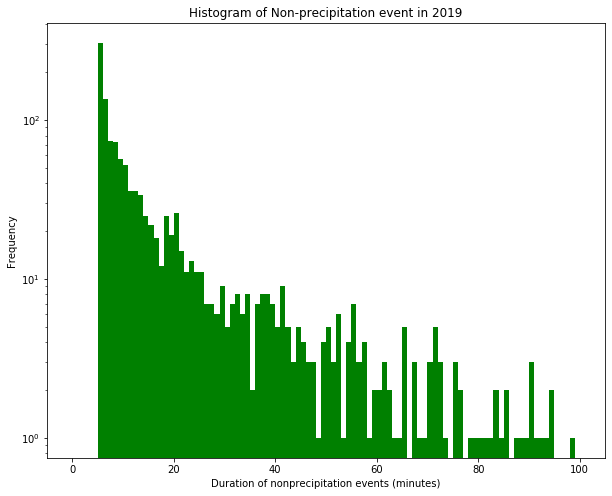
\includegraphics[width=150mm]{nonprecip_hist_5min.png}
	\caption{This is a histogram for the duration of a non-precipitation event, which is to say the gap between two precipitation events. It also follows the pattern of having lots of the non-precipitation events be close to the minimum non-precipitation event of 5 minutes. It does look like that there are more non-precipitation events that lasts longer than say 40 minutes compared to the precipitation events. }
\end{figure}
\begin{figure}[h]
	\centering
	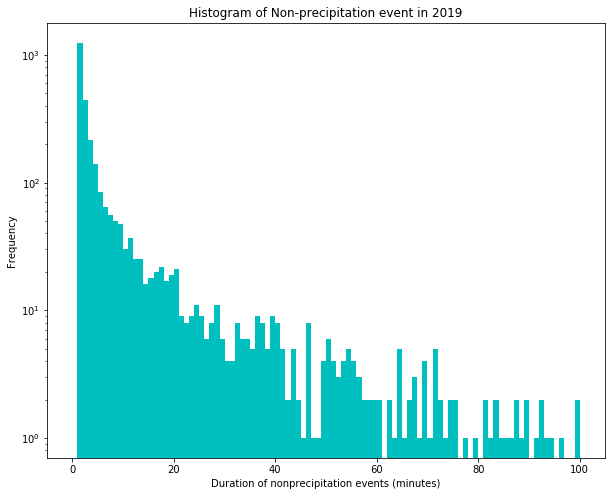
\includegraphics[width=150mm]{nonprecip_hist_1min.png}
	\caption{This is a histogram for the duration of a non-precipitation event, which is to say the gap between two precipitation events. Most events do seem to lie close to the minimum duration of 1 minute. }
\end{figure}
\end{document}